\chapter {Análisis del sistema}

\section{Definición del problema}
\begin{paragraph}
	Hoy en día, aún hay muchas compañías que siguen teniendo dos equipos diferenciados dentro el departamento de IT. Systemas o Operaciones y Desarrolladores. Ya hemos visto en la introducción que esto a la larga causa problemas y no es la forma más rápida y eficiente de desarrollar software. \\
	Trabajo como Administrador de Sistemas en una empresa pequeña y contínuamente aparecen problemas. Es por eso que se ha decidido adoptar un enfoque DevOps par el desarrollo del software. En este cambio están implicados ambos departamentos ya que es responsabilidad de ambos que los cauces de desarrollo y despliegue funcionen correctamente. \\
	En mi compañía la Infraestructura donde se alojan los proyectos, se configura manualmente haciendo prácticamente imposible una replicación de ésta en caso de que sea necesario. También las subidas de proyectos y ejecución de tests no están automatizados y cada desarrollador se encarga de ejecutar los tests en local. Ésto implica discrepancias varias entre el equipo de operaciones y el de desarrolladores. Es por esto que se hace necesario la adoptación de técnicas DevOps como IaaC, CI y CD en la empresa.
\end{paragraph}
\section{Que se pretende resolver}
		\begin{itemize}
			\item Todos los problemas que involucra la configuración manual de infraestructura.
			\item Ralentización de desarrollo de software, al no tener los cauces automatizados.
		\end{itemize}
\section{Casuísticas que se dan y como se resuelve cada una}
		\begin{itemize}
			\item \textbf{Problema 1}: \textit{Recreación ante fallo total o réplica de infraestructura}. Ante un fallo total de la infraestructura o replicación para propósitos de testing, con los sistemas actuales sería imposible, ya que dada la configuración manual de cada uno de los servidores, sería imposible replicar al 100% el estado de los servidores. 
			\item  \textbf {Solución 1}: Al adoptar IaaC, la infraestructura estaŕá codificada en ficheros de configuración bajo control de versiones. Pudiendo recrear la infraestructura bajo demanda en cualquier momento y asegurándonos de que sea la misma al 100%.
			\item \textbf{Problema 2}: \textit{Diferencias entre servidor de desarrollo y producción}. Al desarrollar en local los desarrolladores, no tienen una réplica de los servidores de producción para poder probar sus cambios. Ésto hace que haya discrepancias entre Sistemas y desarrolladores puesto que puede funcioanar en local con una configuración dada pero no en producción. 
			\item \textbf {Solución 2}: Al estar la infraestructura de cada aplicación codificada y bajo control de versiones, será sencillo replicar el entorno de producción en un entorno test para el desarrollo de aplicaciones.
			\item \textbf{Problema 3}: \textit{Petición de subidas a producción}. Al no existir cauces de integración o despliegue, no se tiene un conocimiento exacto de qué comportamiento va a tener la aplicación en producción. Ésto y la necesidad de hacer peticiones al equipo de sistemas para subir nuevas versiones a producción ralentizan el desarrollo del software.
			\item \textbf{Solución 3:} Al tener el desarrollador un servidor réplica de producción para desplegar las aplicaciones, sabe perfectamente el comportamiento que va a tener en producción, puesto que son entornos idénticos. Ésto y los cauces CI-CD solucionan el problema.
		\end{itemize}

\section{Tipos de usuario}
	\begin{paragraph}
		Adoptando la filosofía DevOps, tanto desarrolladores como sysadmins debería adoptar el mismo rol. Sin embargo, en una empresa en la cual crean y configuran sus propios servidores sin contratar servicios externos (como Azure DevOps, AWS...) se crea la necesidad de crear y configurar la infraestructura que va a alojar toda la infraestructura necesaria para el desarrollo cada aplicación. Es por esto que se distinguen entre dos tipos de usuarios: \textbf{Desarrolladores} y \textbf{Sistemas + Desarrolladores}.  
		
		\begin{itemize}
			\item \textbf{Desarrolladores}. Este tipo usuario tiene las siguientes necesidades:
				\item Poder construir una infraestructura para el desarrollo de aplicaciones bajo demanda. [RF 1]
				\item Poder integrar cambios a las aplicaciones. [RF 2]
				\item Poder tener feedback de el estado de la aplicación tras el despliegue. [RF 3]
				\item Conocer la configuración del servidor donde se aloja la aplicación web. [RF 4]
			\item \textbf{Desarrolladores + Sistemas}
				\item Poder construir una infraestructura para el desarrollo de aplicaciones bajo demanda. [RF 1]
				\item Poder integrar cambios a las aplicaciones. [RF 2]
				\item Poder tener feedback de el estado de la aplicación tras el despliegue. [RF 3]
				\item Conocer la configuración del servidor donde se aloja la aplicación web. [RF 4]
				\item Poder desplegar la infraestructura completa que aloja la infraestructura para las aplicaciones. [RF 5]
				\item Poder conocer la configuración de la infraestructura. [RF 6]
		\end{itemize}
	
		Estos historias de usuario representan la funcionalidad final del proyecto, con un nivel de abstracción muy alto. En la siguiente sección, se desgranarán estas historias para definir de forma precisa los requisitos funcionales. \cite{ReqF:online} 
	\end{paragraph}

\section{Especificación de requisitos}
	\label{erf}
	\begin{paragraph}
		A continuación se detallan los requisitos funcionales de este proyecto. 
		\begin{itemize}
			\item Construir y desplegar infraestructura para el desarrollo de aplicaciones bajo demanda. [RF 1]
			\item Poder integrar cambios en las aplicaciones de forma autónoma [RF 2]
			\item Conocer el estado de la aplicación una vez hecho el despliegue [RF 3]
			\item Conocer la configuración del servidor donde se aloja la aplicación web. [RF 4]
			\item Poder desplegar la infraestructura completa que aloja la infraestructura para las aplicaciones a través de ficheros de configuración. [RF 5]
			\item Conocer en todo momento la configuración del servidor [RF 6]
			\item Poder desplegar la infraestructura rápidamentte ante un error catastrófico [RF 7]
			\item Realizar tareas de mantenimiento en los servidores con tareas automatizadas [RF 8]
			\item Crear máquinas virtuales bajo demanda con tareas automatizadas y ficheros de configuración [RF 9]
			\item Modificar la configuración de los firewall con tareas automatizadas [RF 10]
		\end{itemize}
	\end{paragraph}

\section{Diagramas}
	\subsection{Diagramas casos de uso}
		\begin{paragraph}
			A continuación se muestran los principales diagramas según los requisitos funcionales descritos en la sección \nameref{erf}.
		\end{paragraph}
	
		\begin{figure}[!hbt]
			\centering
			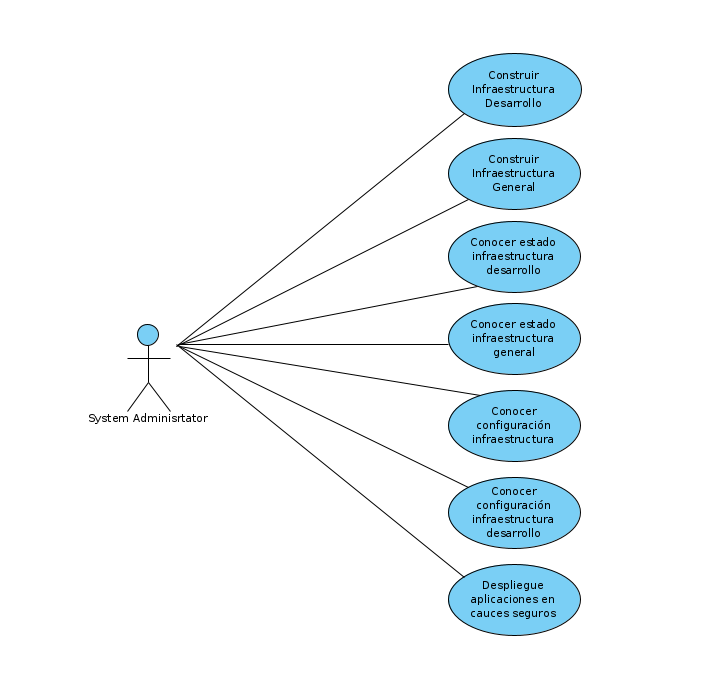
\includegraphics[scale=0.4]{imagenes/Analisis/casos_uso_administrador.png}
			\caption[Casos de uso Administrador]{Casos de uso \cite{casosuso:online}} 
			\label{Casos de uso Administrador}
		\end{figure}
	
		\begin{figure}[!hbt]
			\centering
			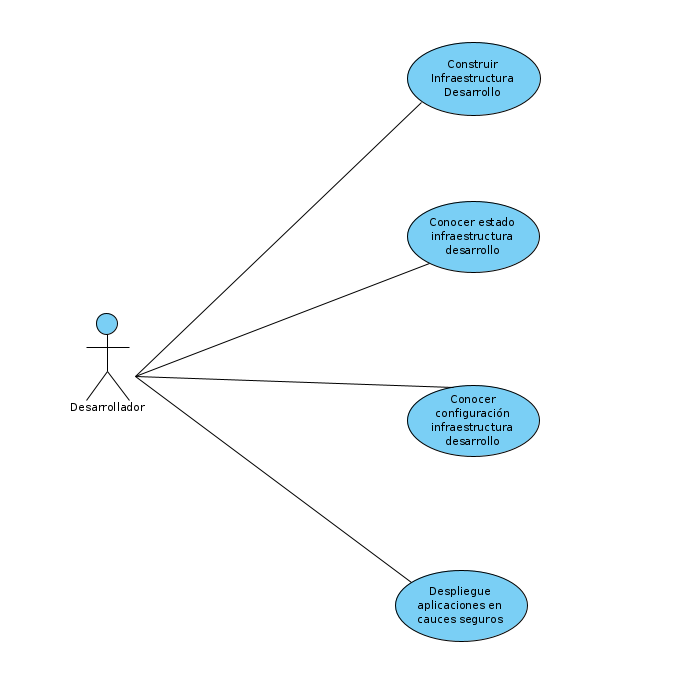
\includegraphics[scale=0.4]{imagenes/Analisis/casos_uso_desarrollador.png}
			\caption[Casos de uso Desarrollador]{Casos de uso \cite{casosuso:online}} 
			\label{Casos de uso Desarrollador}
		\end{figure}
	
	\subsection{Diagramas de secuencia}
		\begin{figure}[!hbt]
			\centering
			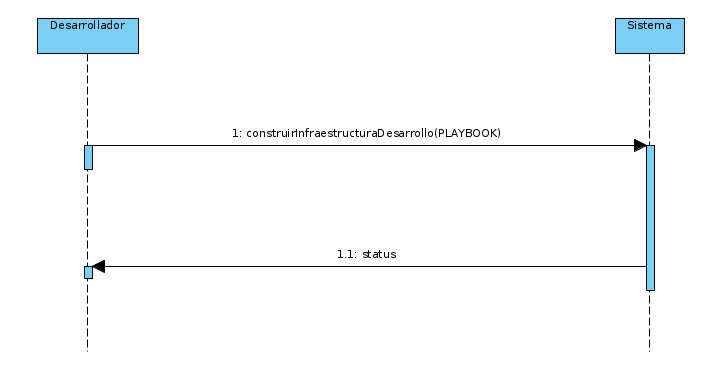
\includegraphics[scale=0.4]{imagenes/Analisis/diagrama_secuencia_desarrollador_1.png}
			\caption[Diagrama secuencia Desarrollador 1]{Diagrama secuencia Desarrollador 1 \cite{diagramasecuencia:online}} 
			\label{Diagrama secuencia_desarrollador_1}
		\end{figure}
		\clearpage
	
		\begin{figure}[!hbt]
			\centering
			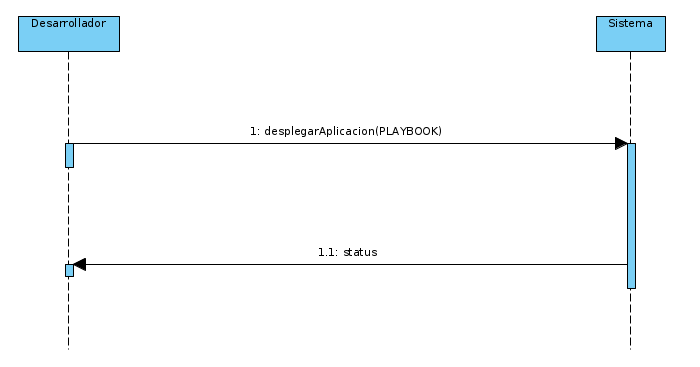
\includegraphics[scale=0.4]{imagenes/Analisis/diagrama_secuencia_desarrollador_4.png}
			\caption[Diagrama secuencia Desarrollador 2]{Diagrama secuencia Desarrollador 2 \cite{diagramasecuencia:online}} 
			\label{Diagrama secuencia_desarrollador_2}
		\end{figure}

		\begin{figure}[!hbt]
			\centering
			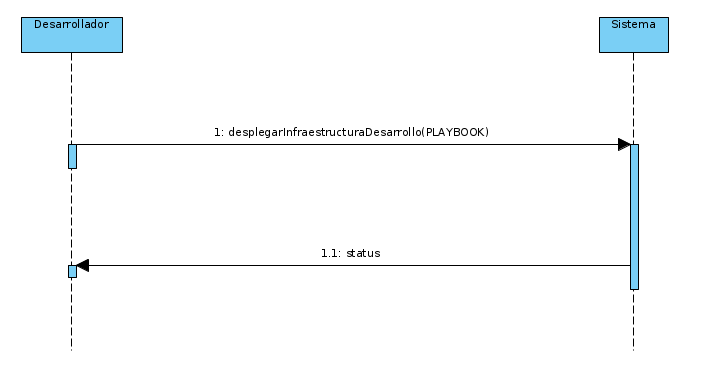
\includegraphics[scale=0.4]{imagenes/Analisis/diagrama_secuencia_desarrollador_3.png}
			\caption[Diagrama secuencia Desarrollador 3]{Diagrama secuencia Desarrollador 3 \cite{diagramasecuencia:online}} 
			\label{Diagrama secuencia_desarrollador_3}
		\end{figure}
	
		\begin{figure}[!hbt]
			\centering
			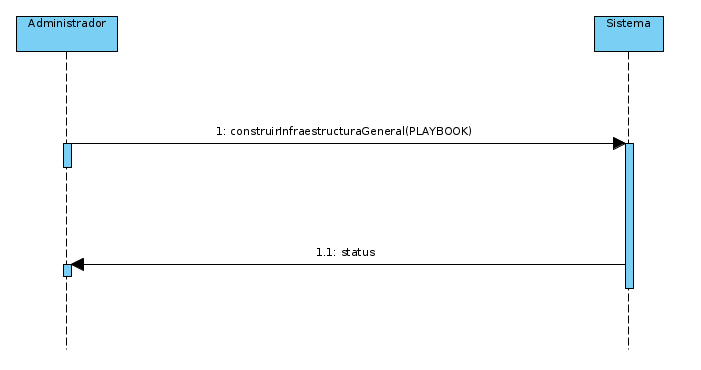
\includegraphics[scale=0.4]{imagenes/Analisis/diagrama_secuencia_administrador_1.png}
			\caption[Diagrama secuencia Administrador 1]{Diagrama secuencia Administrador 1 \cite{diagramasecuencia:online}}
			\label{Diagrama secuencia_administrador_1}
		\end{figure}
		\clearpage
		
		\begin{figure}[!hbt]
			\centering
			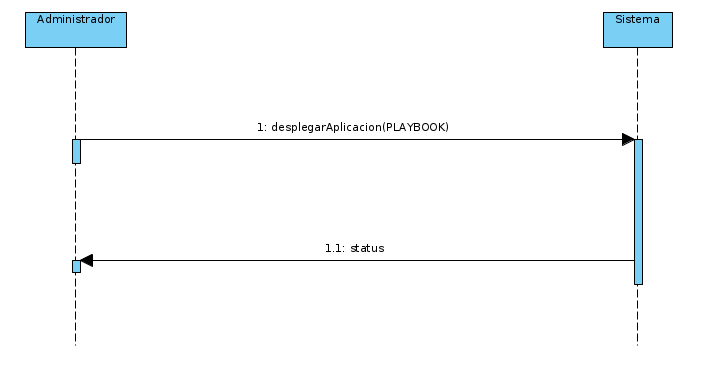
\includegraphics[scale=0.4]{imagenes/Analisis/diagrama_secuencia_administrador_2.png}
			\caption[Diagrama secuencia Administrador 2]{Diagrama secuencia Administrador 2 \cite{diagramasecuencia:online}}
			\label{Diagrama secuencia_administrador_2}
		\end{figure}
	
		\begin{figure}[!hbt]
			\centering
			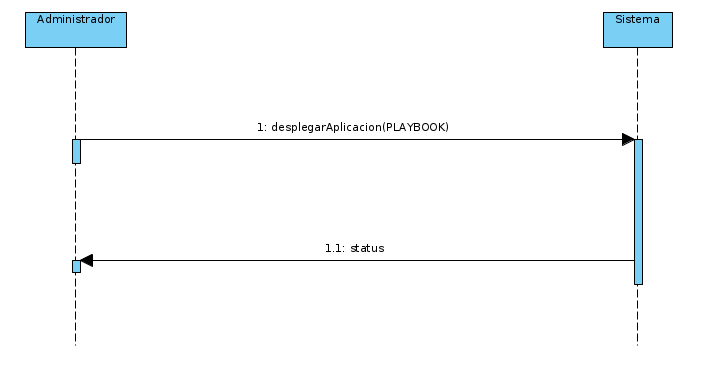
\includegraphics[scale=0.4]{imagenes/Analisis/diagrama_secuencia_administrador_2.png}
			\caption[Diagrama secuencia Administrador 3]{Diagrama secuencia Administrador 3 \cite{diagramasecuencia:online}}
			\label{Diagrama secuencia_administrador_3}
		\end{figure}
		
	
\section{Arquitectura del Sistema}
	\subsection{Servidores Físicos}
		\begin{paragraph}
			Al trabajar en una empresa de hosting, he tenido la suerte de contar con 3 servidores bare metal para el desarrollo de este proyecto.Las características técnicas de los servidores se pueden consultar en \nameref{servidores_bare_metal}.
		\end{paragraph}
	\subsection{Infraestructura objetivo}
		\label{InfraestructuraObjetivo}
		\begin{paragraph}
			Este proyecto pretende crear una infraestructura robusta para una pequeña empresa que se dedique al desarrollo del software. Ésta infraestructura debe ser robusta al igual que segura, con lo que ha de proporcionar firewalls redundantes y algún mecanismo para proporcional alta disponibilidad en las aplicaciones web.  A continuación se muestra la infraestructura objetivo.
		\end{paragraph}
	
		\begin{figure}[!hbt]
			\centering
			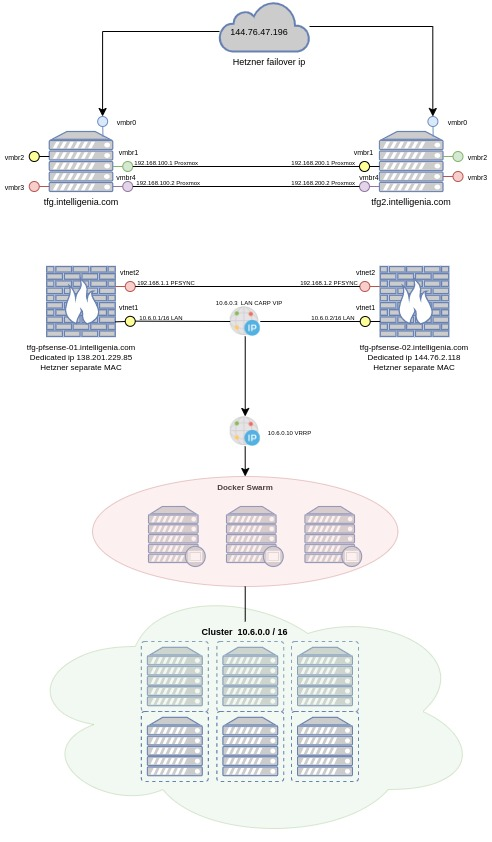
\includegraphics[scale=0.75]{imagenes/Analisis/diagrama.jpg}
			\caption[Infraestructura Objetivo]{Infraestructura Objetivo }
			\label{Infraestructura_objetivo}
		\end{figure}
	\clearpage
	
\section{Metodología de desarrollo}
	\begin{paragraph}
		Todo proyecto software debe tener una organización y unas etapas de desarrollo bien definidas. En esta sección se pretende explicar la metodología de desarrollo elegida para realizar este proyecto. \\
		Se ha tratado este proyecto como cualquier otro proyecto software. Para la organización y el control de versiones se ha elegido Github, un software basado en git originalmente creado para el control de versiones. Actualmente, GitHub ofrece múltiples servicios, como almacenamiento, gestión de paneles de trabajo, registry, integración con mútliples tecnologías... \\
		En cuanto a la metodología de desarrollo, se ha optado por un desarrollo basado en Milestones. Cada Milestone está compuesto por Issues y estos están etiquetados y asignados a personas. A continuación se explican con mayor detalle estos conceptos.
	\end{paragraph}

	\subsection{Milestones}
	\label{milestones}
	\begin{paragraph}
		Los Milestones o Hitos en castellano, corresponden con estados finales deseados de la aplicación. Sabiendo esto, podríamos crear un Milestone por ejemplo: "Servidores configurados a través de ficheros de configuración Ansible". Esto será un estado final deseado para nuestra aplicación o proyecto. Para que un hito quede totalmente realizado, deben estar completos todos los issues marcados como esenciales para el hito. Un hito está compuesto por issues. A continuación se muestran algunos milestones creados en este proyecto, en el panel de administración github.
		
		\begin{figure}[!hbt]
			\centering
			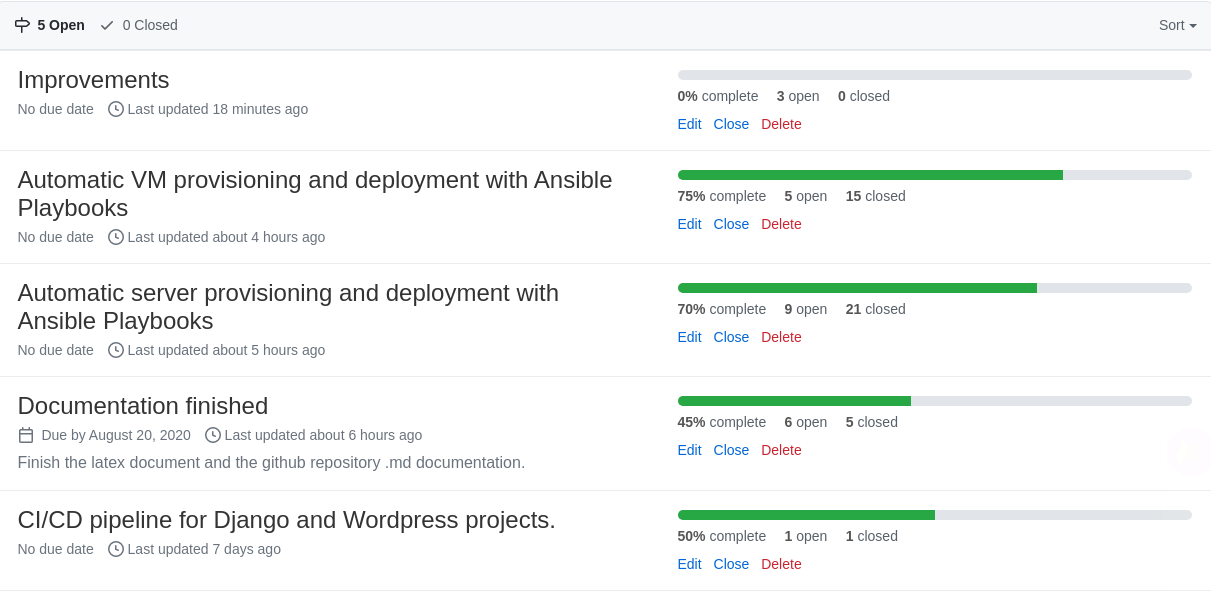
\includegraphics[scale=0.37]{imagenes/Analisis/milestones.png}
			\caption[GitHub milestones]{GitHub milestones}
			\label{github_milestones}
		\end{figure}
	\end{paragraph}
	\subsection{Issues}
	\begin{paragraph}
		Como ya hemos visto, los issues forman parte de los hitos. Es una forma de desgranar el problema. Siguiendo el ejemplo anterior, si tenemos un hito: "Servidores configurados a través de ficheros de configuración Ansible", podemos desgranar el siguiente en distintos issues, que serían tareas más sencillas que hay que realizar para completar el hito. Por ejemplo, algunos issues serían: 
		\begin{itemize}
			\item Crear estructura directorios Ansible.
			\item Instalar paquetes en servidor a través de ficheros de configuración Ansible. \textbf{Core}
			\item Configurar interfaces de red a través de ficheros de configuración Ansible. \textbf{Core}
			\item Instalar ISO en servidor a través de ficheros de configuración Ansible. \textbf{Core}
			\item Instalar certificados SSL a través de ficheros de configuración Ansible. \textbf{Mejora}
		\end{itemize}
	
		Y así seguiríamos creando issues según creamos que van a ser necesarios para completar el hito en cuestión. \\
		En la sección  \nameref{milestones} hemos hablado que los issues tienen etiquetas. En la lista anterior por ejemplo, únicamente tenemos dos etiquetas que nos indican en este caso si son issues imprescindibles para el hito o simplemente mejoras. Gracias a estas etiquetas, podemos distinguir entre distintos tipos de issues y asignar mayor o menos prioridad por etiqueta. También gracias a Github, cada issue puede ser asignado a un desarrollador del proyecto. A continuación se muestra un ejemplo del panel de Github para mostrar los issues, etiquetas y hitos. \\
		Como se puede comprobar, el sistema de etiquetas y asingación de issues a desarrolladores, es más que suficiente para manejar proyectos. Permite asignar prioridades, agrupar issues en hitos y escribir comentarios en cada issue / milestone. 
		
			\begin{figure}[!hbt]
				\centering
				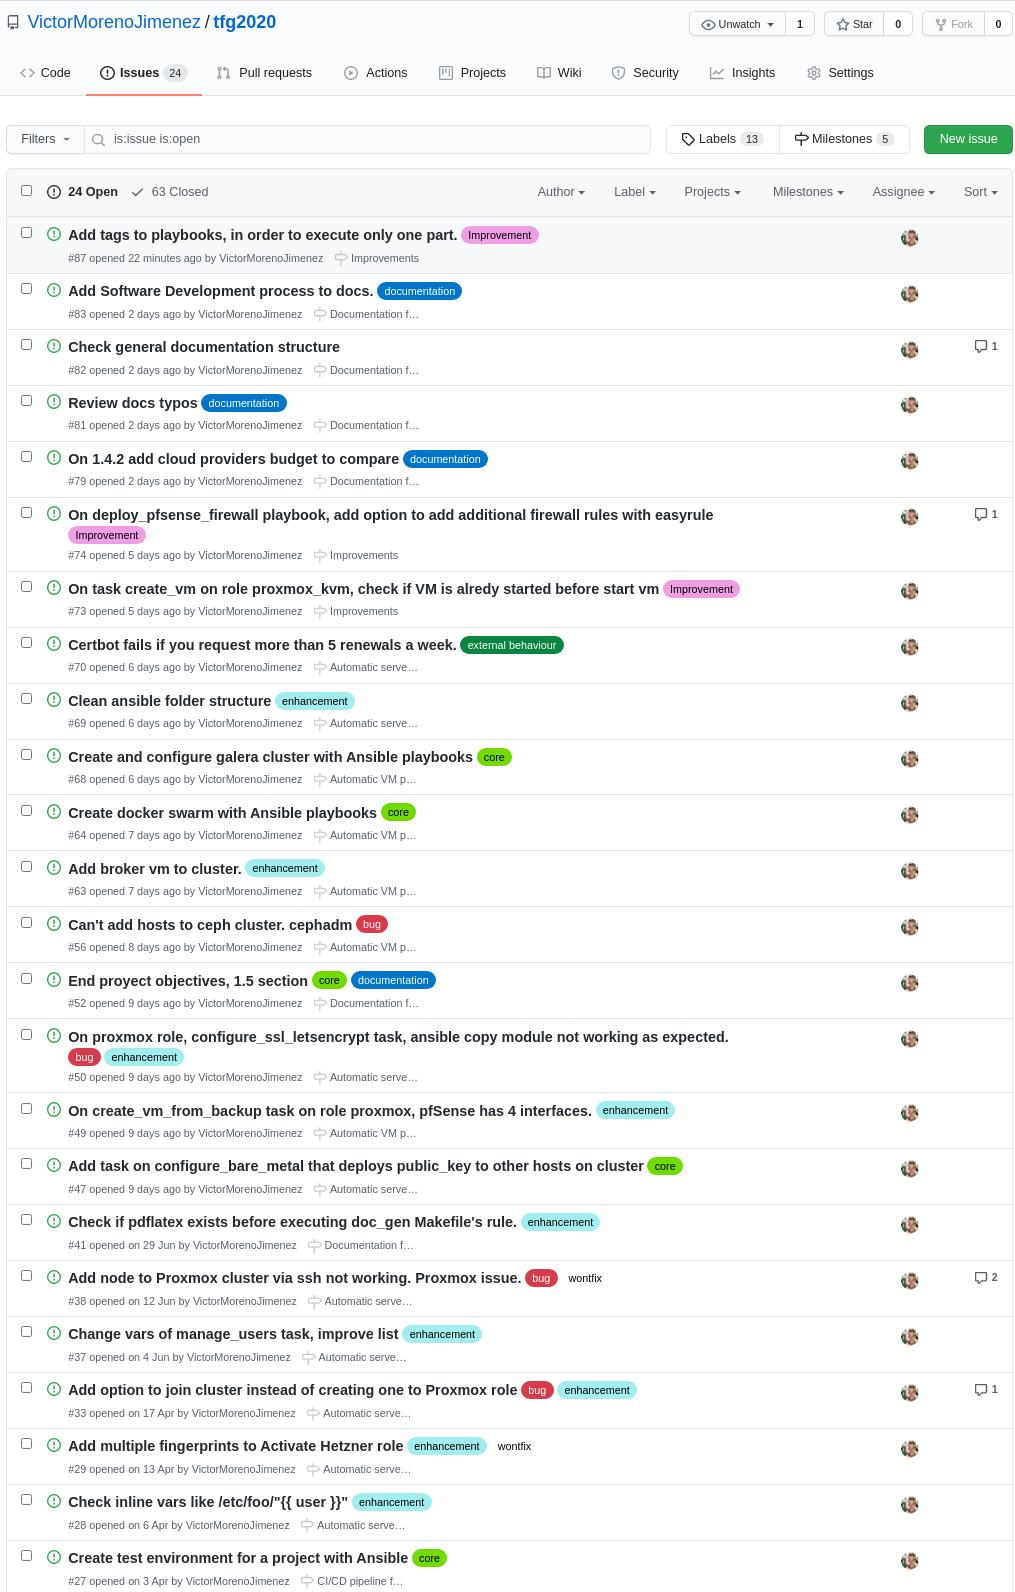
\includegraphics[scale=0.44]{imagenes/Analisis/githubissues.jpg}
				\caption[GitHub panel]{GitHub panel}
				\label{github_issues}
			\end{figure}
	\end{paragraph}
	\clearpage


	
	
	